% Pacotes
\documentclass[12pt]{article}
\usepackage{adjustbox}
\usepackage[utf8]{inputenc}
\usepackage{amsmath}
\usepackage{hyperref}
\usepackage{sbc-template}
\usepackage{fancyvrb}
\usepackage{amsfonts}
\usepackage{amsmath}
\usepackage{pdfpages}
\usepackage{graphicx,url}


\sloppy

\title{Relatório - Xadrez em Racket}

\author{Ricardo Henrique Brunetto\inst{1}}


\address{Departamento de Informática -- Universidade Estadual de Maringá (UEM)\\
	Maringá -- PR -- Brasil
	\email{ra94182@uem.br}
}

\begin{document}

	\maketitle

	\resumo{}

  \section{Introdução}
	O presente documento é um relatório do desenvolvimento de um jogo de Xadrez na
	linguagem funcional Racket para a disciplina 6902 - Paradigma de Programação Lógica
	e Funcional, ministrada pelo professor Dr. Wagner Igarashi para a turma de 2015
	de Bacharelado em Ciência da Computação pela Universidade Estadual de Maringá.

	Neste relatório serão abordadas seções conforme socilitado na especificação do trabalho,
	que pode ser encontrada em anexo a este documento.

	\section{O Jogo}
	O jogo foi desenvolvido em Racket com uso do editor de textos Atom e da IDE DrRacket.

	Foi desenvolvido um jogo de Xadrez onde o 

	\bibliographystyle{sbc}
	\bibliography{references}

	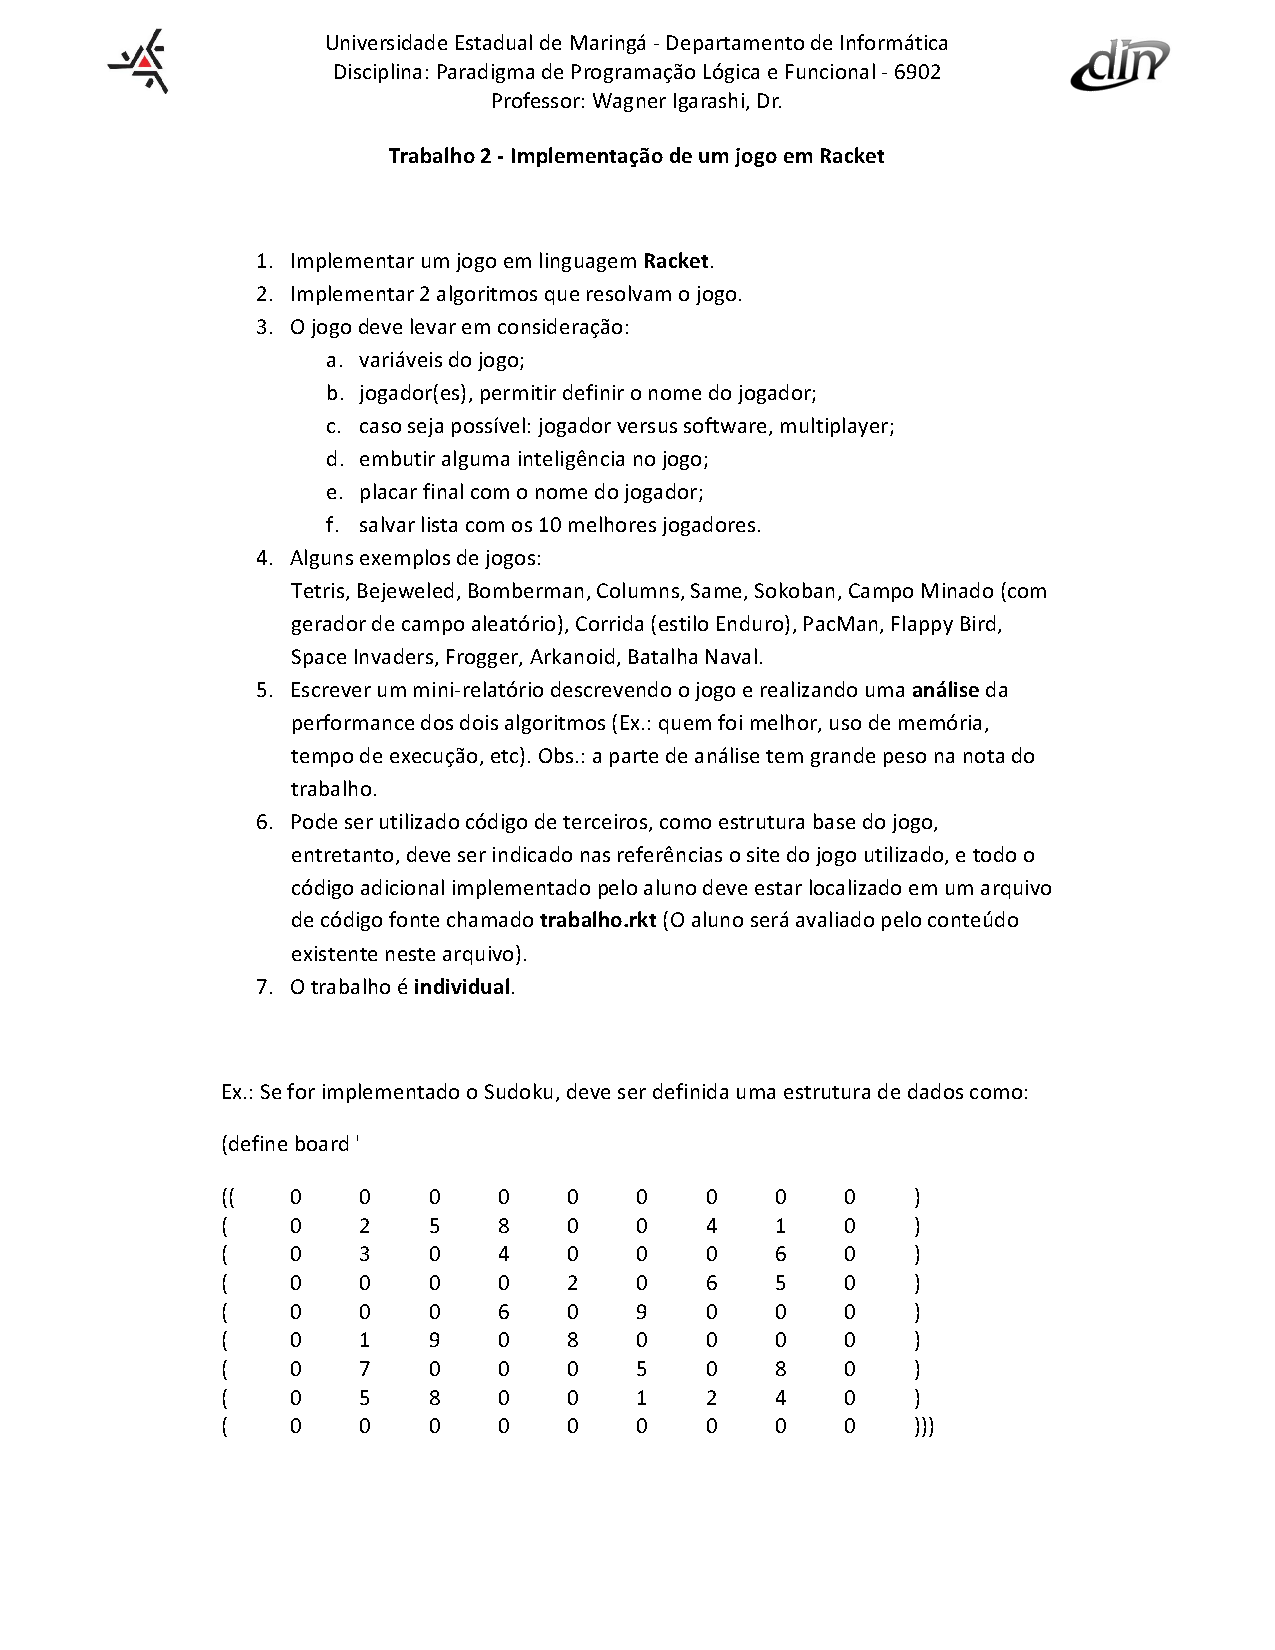
\includepdf[pages=-]{especificacao}

\end{document}
